\section{Edge computing}\label{sec:lit:edge-computing}
Projections performed by Forbes suggest that by 2025, more than 75 billion Internet of Things(IOT) devices will be connected to the Internet.\cite{forbesiot}
As the devices at the edge become more computationally capable and more numerous, it becomes imperative to share the computational load not only across the cloud services, but across the devices themselves.
Furthermore, a large portion of these devices, such as home automation, do not require a connection to the cloud in the first place.
Instead they require a connection to the edge IOT hub, or need the cloud service only to establish or broker communication with another IOT device.
Edge computing is a subset of IOT research, which concerns itself with distributing the computational load across the devices at the edge of the of the network. \cite{satyanarayanan2017emergence}
\begin{figure}[h]
    \centering
    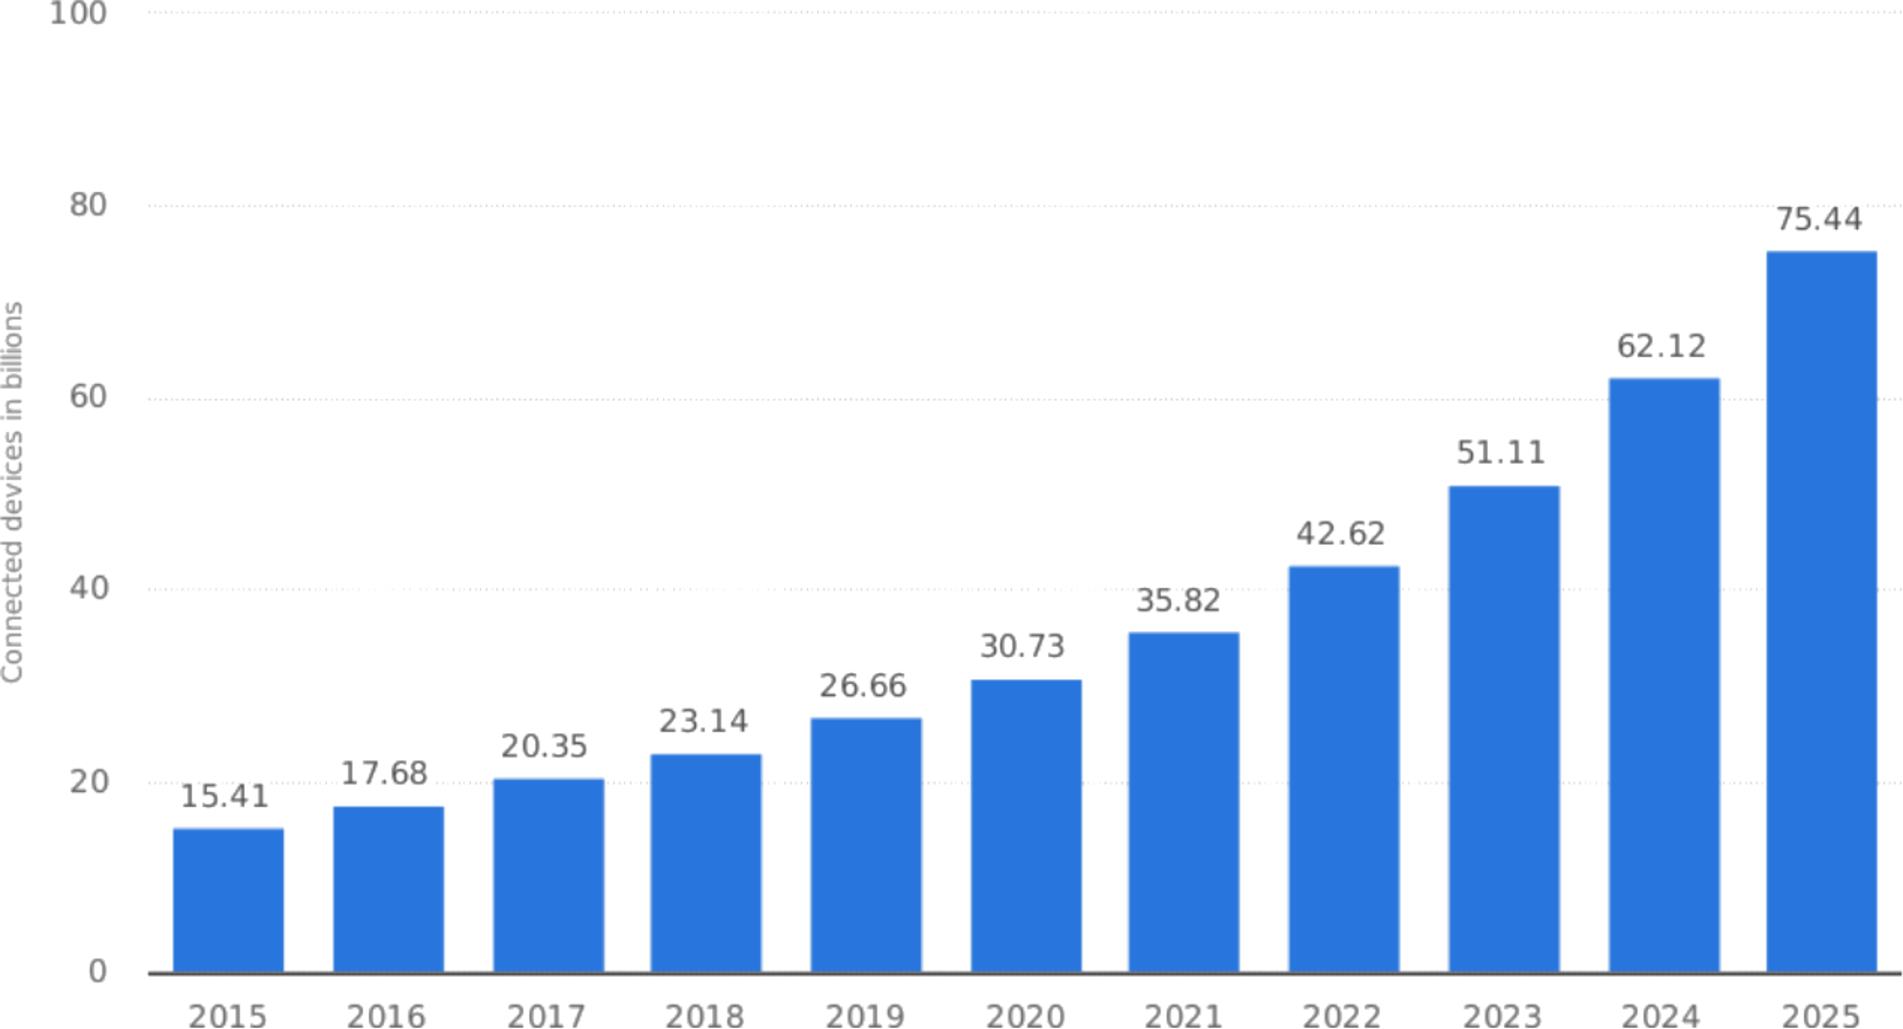
\includegraphics[width=0.8\linewidth]{img/iot_statistics.pdf}
    \caption{Projected number of IOT devices worldwide.\cite{forbesiot}}
    \label{lit:fig:1}
\end{figure}

This change in computational strategy may seem inconsequential at first.
However, upon deeper reflection it becomes clear that this is a major paradigm shift which brings IOT closer to the sensor network world it is often compared with.
While pioneering work in IOT always assumed a one or two-way communication between the IOT device and the cloud service, utilizing TCP/IP as an end-to-end protocol, it is becoming clear that this approach is unsustainable, and is often undesirable.
This communication model has clear disadvantages in wasted communication, computation, and privacy.
Furthermore, the rigid computation communication model is not flexible enough to support devices which are beyond the edge of the TCP/IP network without resorting to ad-hoc routing. \cite{gagliardi2011content}

The first attempt to address the bandwidth and latency issues arising with widespread IOT adoption came in form of content delivery networks (CDNs).\cite{gagliardi2011content}
CDNs circumvent the generic cloud information delivery problems by placing transparent caches geographically spread across the application domain as shown in Figure \ref{lit:fig:2}.
When a user or an IOT device makes a request for an object, this request is forwarded to the nearest CDN node for processing.
If the node contains the object in its cache it is immediately forwarded to the requestee.
Otherwise a request for the object is forwarded to the centralized cloud data store, and returned to the requesting device, as well as placed in the local cache.
This approach has the advantage of moving the data closer to the end user, thus reducing latency, and taking advantage of geographical locality.
Another advantage of this method is the added resiliency of the CDN architecture to a single point failure.
If a local cache node fails, its userbase can be forwarded to another node, although incurring additional latency.
Additionally, if a centralized data store becomes unreachable, the local cache nodes can to some extent mask it's outage by forwarding the data available locally.
This approach does have some drawbacks.
While it makes it easier to enable faster transactions regarding data, it is not trivial to move application logic to the local cache nodes.
Furthermore, the CDN methodology, still relies on a central mediator for device communication, even if the devices are located in the same room.

\begin{figure}[h]
    \centering
    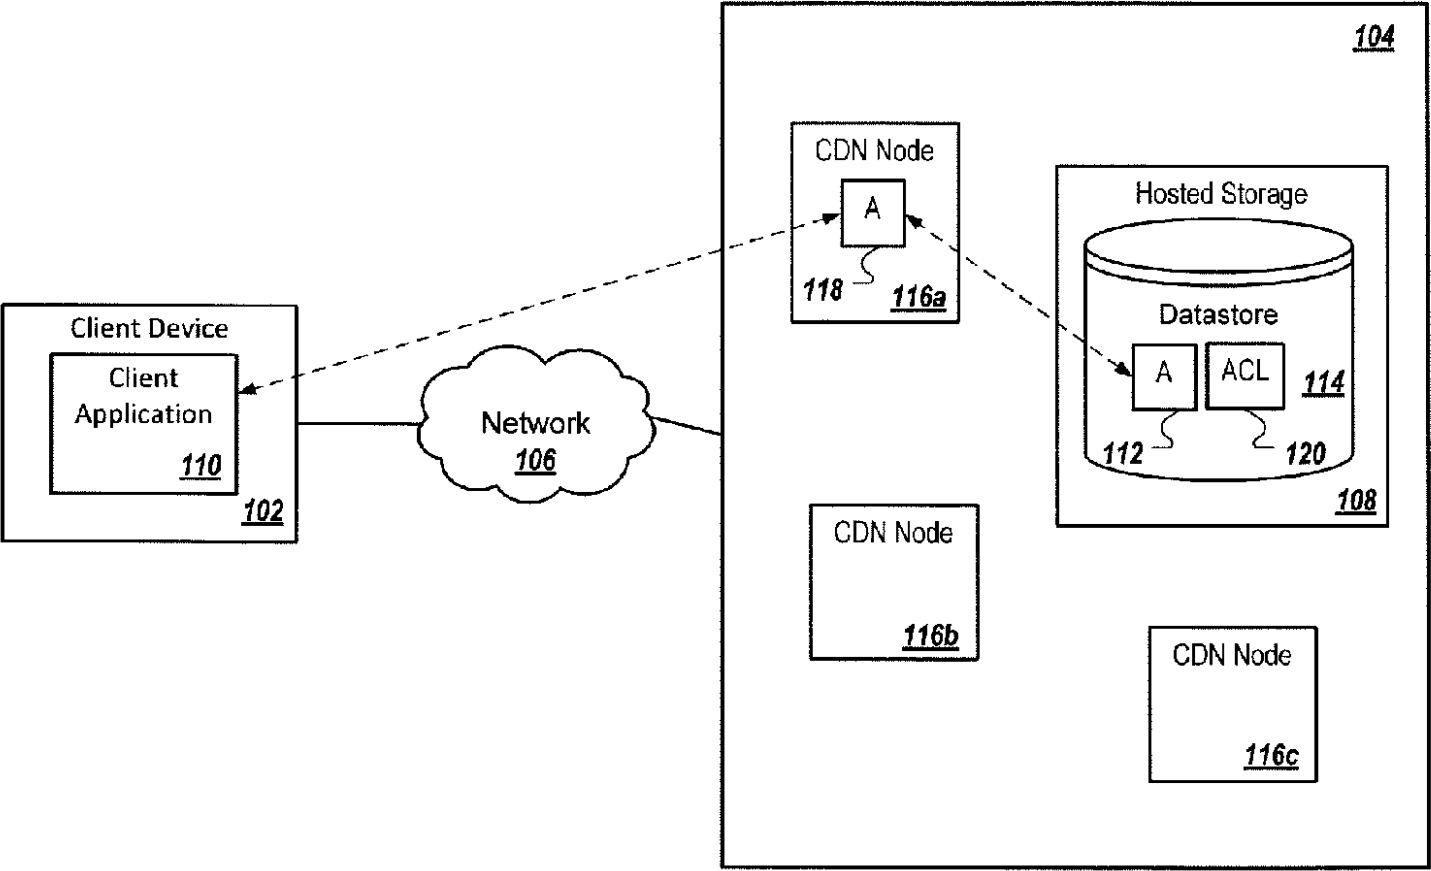
\includegraphics[width=0.6\linewidth]{img/cdn.png}
    \caption{Content delivery network architecture.
    As described in the Google patent.\cite{gagliardi2011content}}
    \label{lit:fig:2}
\end{figure}

In an attempt to support a more diverse IOT ecosystem, current research is focused on moving the cloud service ever closer to the edge of the network.
Since the majority of IOT devices are located within one hop of the Internet, the next logical place to locate a content provider is at the wireless basestation.\cite{satyanarayanan2017emergence} These servers, commonly referred to as cloudlets or fog servers, are collocated with various wireless basestations, which allows them to provide a location specific service to the user without using the Internet.
This approach also provides uniform access and simplifies intercommunication between a variety of devices, including those that don't use TCP/IP. Unlike the localized cloud cache approach relied on by the CDNs, fog servers are built with the notion of moving not only data but also the application logic to the edge of the network.
To facilitate inter-device communication between the devices using differing wireless protocols, fog servers can no longer rely on TCP/IP routing.
Instead, TCP/IP becomes yet another transfer protocol along with Bluetooth, Zigbee, 3g etc, with routing between the devices implemented as a software service.\cite{edgeiot} A few use-cases of such technology are already found in industry.
Examples of these include airline/bus in-flight entertainment, and shopping mall directory apps.
A block diagram of this infrastructure is shown in figure \ref{lit:fig:3}.
In the future, emerging technologies which are sensitive to latency, such as virtual and augmented reality will benefit from fog computing, since it's inherently lower latency than the cloud counterparts.

\begin{figure}[h]
    \centering
    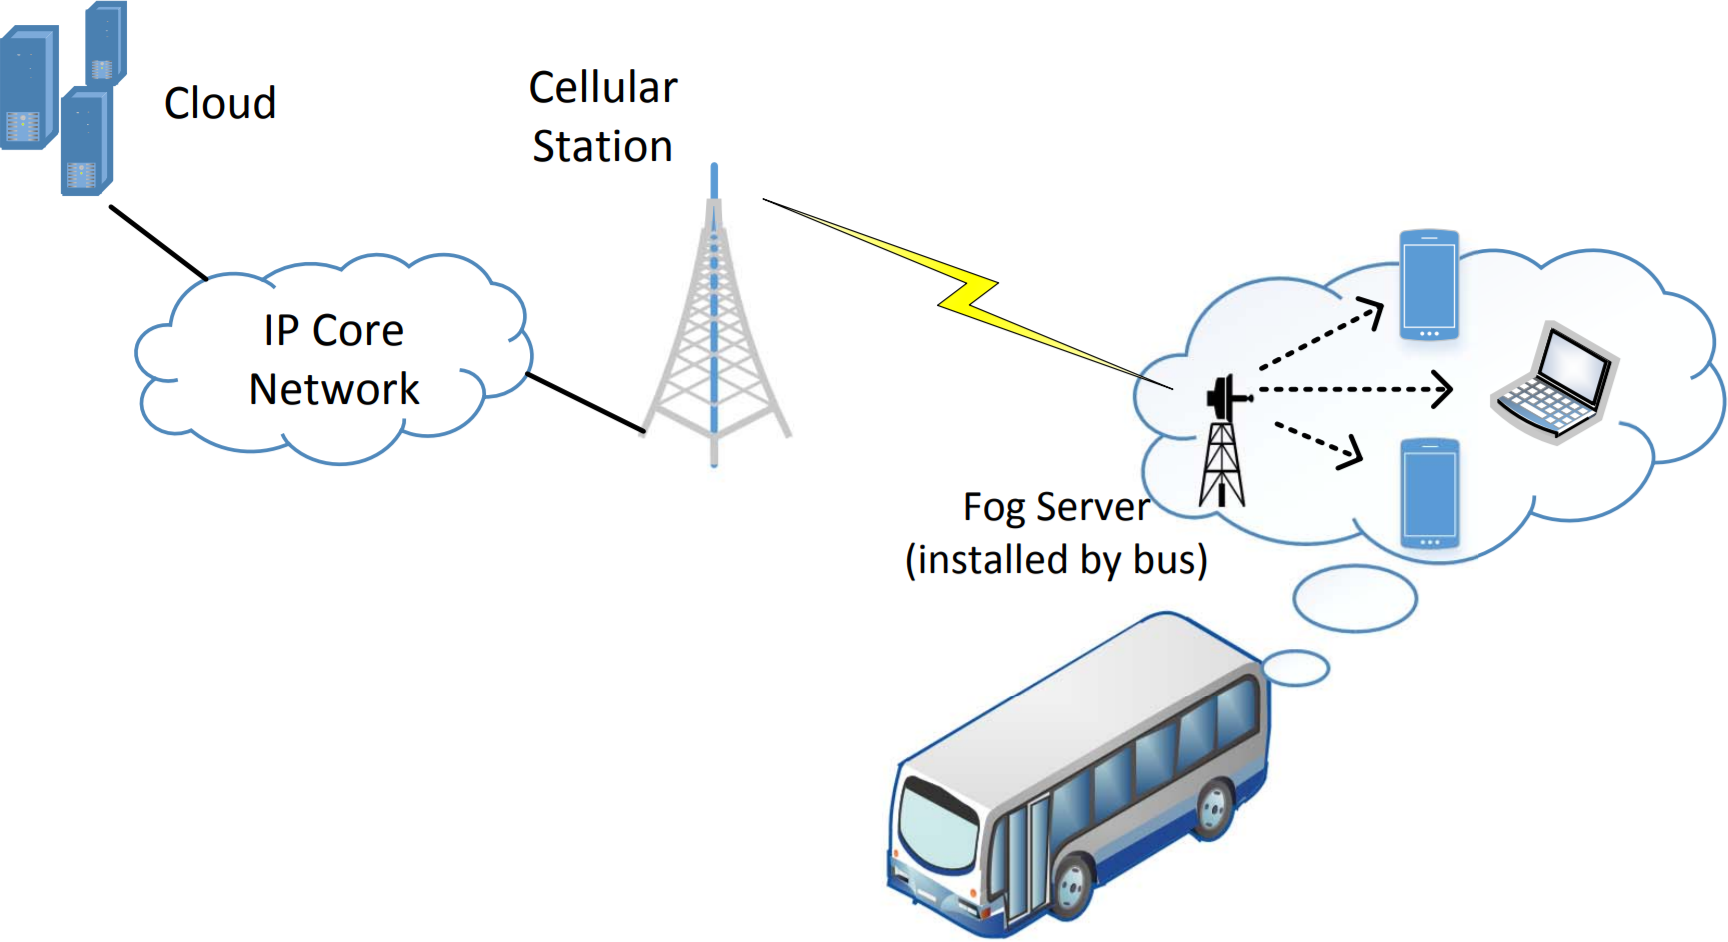
\includegraphics[width=0.6\linewidth]{img/fog_comp.png}
    \caption{Fog computing use in transportation.
    The bus cloudlet provides a cache for common data such as commuter schedules and traffic information, while routing other queries to the Internet.\cite{edgeiot}}
    \label{lit:fig:3}
\end{figure}

With the architecture for low latency communication between the edge devices and the fog provider established, the state of the art in edge computing research is focused on intelligent sharing of the computational resources in the fog system.
Edge servers generally have far more computational capacity than the edge device, however, they service many such devices.
Additionally, due to the fickle nature of radio links connecting the edge device to the fog service, the work sharing protocol must be able to cope with link and packet loss.
Finally, in the case of battery powered devices, the energy cost of transmitting the computational job, and receiving its result may exceed the cost of performing the computation locally.
Finally, with mobile edge nodes, such as smart phones, and smart cars, computational offloading algorithms must be able to handle constant network reconfigurations as the edge nodes enter and leave the fog server geographical area.
A number of algorithms have been proposed for efficient and robust computational sharing in fog environments. \cite{oueis2015fog} \cite{wang2015mobiscud} \cite{wang2013mobile}

Napali fits in-between the CDN and Fog server architectures.
The power quality disturbances are generally localized to a specific area, so a sink placement which covers a small geographical area is preferred in order to reduce latency and reduce unnecessary communication with the centralized cloud location.
Furthermore, sink-driven measurement rate allows the OPQ Box to dynamically scale the computational and communication overhead.
Finally the event, classification and analysis are similar to the computational offloading strategies currently under development in the edge computing field.

\section{Distributed Power Quality Monitoring}\label{sec:distributed-power-quality-monitoring}

Power quality monitoring is a long established field in the smart grid domain.
However, the vast majority of research so far has focused on single point power quality monitoring.\cite{silva2017development} Such research has extremely useful applications in industry, since it allows one to ascertain the absolute quality of the delivered power at a given location.
However, since power quality disturbances can originate both from local sources and from gridwide disturbances, single point monitoring is not particularly useful for smart grid research.
Several projects have developed a distributed approach to power quality monitoring, the most prominent being the FNet project and the Power Standard Lab PQube deployment.


The FNet project designed, manufactured and deployed a Phase Measuremnt Unit (PMU), across over 300 locations across the united states.\cite{zhang2010wide} PMU devices plug into an outlet, and sample the power line voltage at the rate of about 1.5kS/s.
The sampling is disciplined by GPS, and as such FNet devices are extremely sensitive to voltage frequency and phase angle.
The precision of the FNet devices is $~0.5mHz$ for frequency and $0.02^{\circ}$ for phase angle.
Collected data is sent to the collection service at 100ms intervals via the Ethernet connection.
Using these devices FNet was able to observe several large power disturbances in the US power grid.
The robustness and sensitivity afforded by the GPS receiver makes this project an excellent source of frequency data across large geographical area, however, the sampling rate of 25 samples per grid cycle is far too low to properly sample fast transients and sags.
Furthermore, FNet provides no methodology for acquiring raw data for event disturbances which it records.

Power Standards Lab (PSL) has been an industry leader in power quality monitoring, and has authored several standards on the topic.
Furthermore, PSL has developed and deployed a large number of power quality monitors called PQube across the world.
The exact number of deployed devices is uncertain since a lot of the devices are deployed industrially and are not available to the public.
However PSL has several publicly available devices, as well as several PQ datasets accessible for smart grid researchers.
PQube devices are an industry standard for power quality monitoring, sampling at $12.8kSps$ for both the voltage and current waveforms.\cite{pqube_spec} Each PQube device is supplied with a NIST certificate of compliance and complies with the IEC 61000-4-7:2002 standard for PQ measurements.
Incidentally, this standard was authored in part by the PSL staff.
Similarly to the FNet PMU, PQube devices are GPS disciplined, additionally the sampling is phase-locked to the voltage waveform allowing for an even more precise metric extraction.
Finally each PQube device is configurable with custom thresholds which allow it to record raw PQ event data for the location it's monitoring.
PQube offers a centralized data collection option with flexible communication schemes ranging from Ethernet to Cellular.
Since PQube devices monitor current in conjunction to voltage, its installation requires it to be placed into the electrical box of the target, by a licensed electrician.\cite{von2014micro} Furthermore, the GPS synchronization requires addition of extra conduit to the electrical box to allow for an antenna.
Finally, since the PQube devices are designed for single location measurements, distributed event detection using the PQube network is particularly difficult, with a lot of low magnitude gridwide events being incomplete or missing.


Unlike the single point monitoring solutions, the Napali framework is incapable of operating as standalone PQ monitor without a cloud sink.
Furthermore, even with the event detection sink, the goal of Napali is to reject local anomalies in order to reduce the communication and computational overhead.
While not as sensitive as the PQube device, the deployment price per unit is two orders of magnitude lower, while providing better sensitivity than compared to the FNet device, when running with GPS.
The ability of OPQ Box nodes to utilize NTP, with WIFI connectivity, means that the OPQ Box deployment is much simpler than the FNet and PSL offering, without requirements of a clear view of the sky or additional wiring for Ethernet and GPS antennas.
Finally, Napali distributed event detection system allows for acquisition of the entirety of the PQ disturbances including in locations where the disturbance has been greatly attenuated by the electrical distance.
Thus, Napali is able to provide a more complete picture of the disturbance propagation throughout the smart grid.

\section{Anomaly detection in Power Quality Monitoring Networks.}\label{sec:anomaly-detection-in-power-quality-monitoring-networks.}

Anomaly detection in PQ monitoring networks remains an active topic of research.
The goal of PQ event detection is to isolate the temporal regions where the voltage or current waveform deviates from the nominal by a given threshold.
In some cases the aim is simply to notify a higher level control system in a realtime manner that a disturbance is taking place.
In other cases, the goal is to acquire the raw disturbance data for off-line analysis.
Most of the detection methods rely on statistics and thresholding in order to detect PQ disturbances.
Most of the literature concerns itself with single point detection, for purposes of protection of equipment downstream.\cite{gu2004statistical}\cite{karimi2000wavelet} \cite{shin2006power} Distributed power quality projects will generally utilize single single point detection across multiple devices in order to reconstruct gridwide propagation.\cite{von2014micro}

With a wide deployment of smart meters, PQ researchers gain access to a networked platform which is perfectly positioned for PQ monitoring.\cite{hoglund2012using}
The major issue for smart meter real time monitoring is bandwidth constraints.
Smart meter deployment is envisioned to communicate via a mesh network with a stationary or mobile base station used for data aggregation.
As such the bandwidth and connectivity is limited, thus requiring methodology which is capable of event detection in such environments.
Generalized local likelihood ratio detection is one method for overcoming these limitations.
This approach requires only a single bit to be forwarded from each smart meter indicating whether a disturbance is taking place or not.
These bits are aggregated at the ``master'' meter, and if their sum exceeds a threshold a higher level control system is notified of the ongoing disturbance.\cite{li2016cooperative} This approach is resilient to bandwidth limitations, and communication instability, however tuning thresholds for each individual meter requires a significant manual effort.

Systems designed for distributed PQ event detection using custom meters are prevalent in literature.
A study at CERN utilized PQube devices with gapless recording which were later analyzed off-line, in order to ascertain the propagation mechanics of PQ events.\cite{kahle2016power} In a realtime domain Shang Li and Xiaodong Wang extended their work in \cite{li2016cooperative} from smart meters to standalone devices, again advocating for single bit statistical based triggering generated by asynchronous meters.\cite{li2013monitoring} Unfortunately their work has never been verified beyond simulation.
The Transimeter project utilized an analog hardware event detector comprised of a high pass filter and a comparator for transient detection.
These devices had two data paths for the voltage waveform, one to the National Instruments DAC board, one to the hardware trigger circuit.
If a trigger circuit detected a transient, a flag was set on the NI DAC, which would in turn instruct the connected PC to send the data to the central server.\cite{daponte2004transientmeter} Unfortunately, the lack of cooperative detection and an inflexible trigger circuit makes this approach unappealing for modern power quality monitoring.
Some of the more exciting work in PQ detection is modeling the most efficient placement of PQ meters in order to provide complete coverage for the power grid. \cite{won2006new} Another is using distributed detection for localization of the event source.\cite{parsons1998direction} \cite{polajvzer2017evaluation}

Napali differs from the smart-meter approach in the use of WiFi for communication, which greatly decreases the communication constraints of the system.
Since the OPQ Box is always connected to the power grid it is monitoring, power concerns are minimal.
This allows Napali to implement more robust computational and communication strategies, not commonly possible with smart meter PQ monitoring.
Since the triggering stream is generated in software, it is possible to switch the detection metrics without redesigning new hardware.
Napali combines both cooperative PQ event detection and PQ event acquisition which makes it useful for future PQ event localization, and propagation research.\cite{parsons1998direction} \cite{polajvzer2017evaluation}
